\documentclass[a4paper]{article}
\usepackage[spanish,es-lcroman]{babel}
\usepackage[utf8]{inputenc}
\spanishdecimal{.}
\usepackage{bm}
\usepackage{amssymb}
\usepackage{mathtools}
\usepackage{amsmath}
\usepackage{geometry}
\usepackage{parskip}
\usepackage{graphicx}
\usepackage{listings}
\usepackage{xcolor}
\usepackage{float}
\usepackage{tikz}
\usepackage{multicol}
\usepackage{enumitem}
\usepackage{subcaption}
\usepackage{animate}
\definecolor{mygreen}{rgb}{0,0.6,0}
\definecolor{mypurple}{rgb}{0.7,0.3,0.7}
\lstset{
	language=Python,
	backgroundcolor=\color{white},
	frame=none,
	%
	basicstyle=\tt,
	commentstyle=\itshape\color{mygreen},
	keywordstyle=\color{magenta},
	identifierstyle=\color{cyan},
	stringstyle=\color{mypurple},
	showstringspaces=false,
	%
	numbers=none,
	%	numberstyle=\color{gray},
	firstnumber = 1,
	stepnumber=2,
	tabsize =2,
	%
	columns=flexible,
	breaklines=true
}
\lstset{
     literate=%
         {á}{{\'a}}1
         {í}{{\'i}}1
         {é}{{\'e}}1
         {ý}{{\'y}}1
         {ú}{{\'u}}1
         {ó}{{\'o}}1
         {ě}{{\v{e}}}1
         {š}{{\v{s}}}1
         {č}{{\v{c}}}1
         {ř}{{\v{r}}}1
         {ž}{{\v{z}}}1
         {ď}{{\v{d}}}1
         {ť}{{\v{t}}}1
         {ň}{{\v{n}}}1
         {ů}{{\r{u}}}1
         {Á}{{\'A}}1
         {Í}{{\'I}}1
         {É}{{\'E}}1
         {Ý}{{\'Y}}1
         {Ú}{{\'U}}1
         {Ó}{{\'O}}1
         {Ě}{{\v{E}}}1
         {Š}{{\v{S}}}1
         {Č}{{\v{C}}}1
         {Ř}{{\v{R}}}1
         {Ž}{{\v{Z}}}1
         {Ď}{{\v{D}}}1
         {Ť}{{\v{T}}}1
         {Ň}{{\v{N}}}1
         {Ů}{{\r{U}}}1      
         {s̄}{{\={s}}}1
         {ñ̄}{{\~{n}}}1
         {Ñ}{{\~{Ñ}}}1
}

\newenvironment{sidefig}[1]
{\noindent\begin{minipage}[c]{#1\textwidth}}
	{\vfill\end{minipage}}
\newcommand{\herefig}[1]{%
\end{minipage}
\hfill
\noindent\begin{minipage}[c]{#1\textwidth} 
	\centering\vfill
}

\author{Celia Rubio Madrigal}
\title{Práctica 3 voluntaria - GCOMP}
%\date{3 de mayo de 2022}

\usepackage{hyperref}

\begin{document}
	\maketitle
	
	\tableofcontents
	
	\vfill
	
	\begin{center}
%		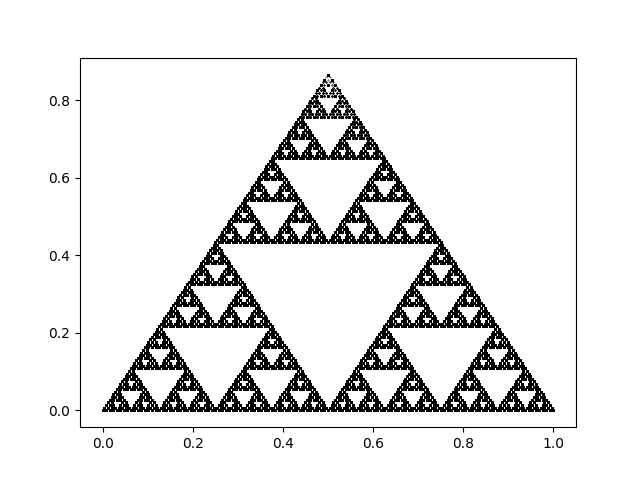
\includegraphics[width=0.7\linewidth]{img/triangle7}

\animategraphics[method=ocg,width=0.45\paperwidth,loop,autoplay]{6}{img/triangle}{0}{8}\renewcommand{\thefootnote}{}\footnote{$^*$Para ver este gráfico en movimiento, se recomienda abrir este PDF en Adobe Reader u Okular.}
	\end{center}
	
	
	\vfill
	\newpage
	
	\section{Introducción}
	En esta práctica vamos a dibujar un fractal, y a calcular su medida de Hausdorff.
	
	En este caso, el fractal escogido es el triángulo de Sierpinski, que es una generalización del conjunto de Cantor para triángulos equiláteros.
	
	Sabemos que su dimensión de Hausdorff real es $\frac{\log 3}{\log 2} \approx 1.585 \pm 0.001 $. Queremos observar cuánto nos acercamos a este valor.
	
	\section{Material usado y metodología}
	
	
	\subsection{Apartado \textit{i})}
	En el primer apartado, vamos a construir el fractal y a representarlo. Tendremos una familia de subconjuntos del fractal en función de un nivel $\ell$, cuyos puntos estarán contenidos en $\ell+1$.
	
	Para $\ell=0$, el conjunto de puntos son los tres vértices del triángulo equilátero de lado 1. Para $\ell$ arbitrario, tomamos todos los triángulos formados en el nivel $\ell-1$. Por cada uno de ellos (de coordenadas $(p_1,p_2,p_3)$), se añadirán estos triángulos a la capa siguiente, donde $m$ es el punto medio:
	\[ \Delta_0 = (p_1 , m(p_1,p_2)), m(p_1,p_3)) \]
	\[ \Delta_1 = (m(p_1,p_2)), p2, m(p_2,p_3)) \]
	\[ \Delta_2 = (m(p_1,p_3)), m(p_2,p_3), p_3) \]

	\subsection{Apartado \textit{ii})}
	En el segundo apartado, calcularemos su dimensión de Hausdorff. Tomando su ${d_0}$-medida de Hausdorff:
	\[ \mathcal{H}^{d_0} = \lim_{\delta\to 0}  \inf{\sum_{i\in I} \delta^{d_0}} \]
	
	Donde $\{U_i\}_{i\in I}$ es un recubrimiento del conjunto de diámetro $\delta$ embebido en $\mathbb{R}^2$.
	
	La $d$ que buscamos es la $d$ ínfima en $d_0$ tal que $\mathcal{H}^{d_0}$ es nula, que es equivalente a la $d$ suprema en $d_0$ tal que $\mathcal{H}^{d_0}$ es infinita.
	
	Sea $\varepsilon=0.01$. Tomaremos un recubrimiento de cuadrados de lado $\frac{1}{n}$, con $n$ entre 1 y $\frac{1}{\varepsilon}=100$. Recorreremos el conjunto de posibles dimensiones, desde 0 (dimensión de los puntos) a 2 (dimensión ambiente). 
	
	Por cada nivel de construcción $\ell$ del triángulo de Sierpinski, por cada $n$ y por cada $d$, contaremos cuántos cuadrados del recubrimiento tienen puntos del fractal. Cuando la medida de Hausdorff (esa cantidad por el volumen) sea menor que $\varepsilon$, entonces pasaremos al siguiente $n$.
	
	Por cada $\ell$ y cada $d$, haremos una gráfica de los valores de esa medida frente a $n$. El resultado que devolveremos será el máximo $d$ para el máximo $\ell$ que hayamos considerado, tal que la medida de Hausdorff del máximo $n$ sea menor que $\varepsilon$. Con el resto de gráficas, podremos comprobar las tendencias de cada medida tomada.

	
	\section{Resultados y conclusiones}
	\subsection{Apartado \textit{i})}
	En la portada de este trabajo se encuentra una animación de todas las figuras para los niveles de 0 a 8. Para $\ell=8$, el triángulo de Sierpinski resultante es el siguiente:
	
\begin{center}
		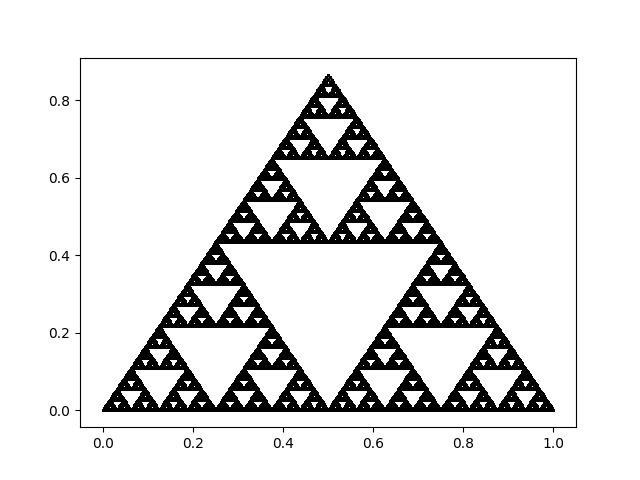
\includegraphics[width=0.5\linewidth]{img/triangle8}
\end{center}
	
	\subsection{Apartado \textit{ii})}
	Por ejemplo, la gráfica del nivel $\ell=6$ llega a $d=1.38\pm 0.01$, y las gráficas, desde $d=0.78$, son las siguientes (izquierda):
	
	\begin{multicols}{2}
		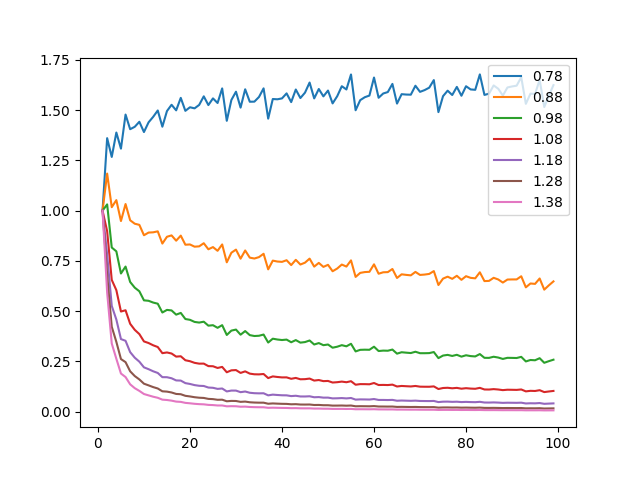
\includegraphics[width=0.95\linewidth]{img/6}	
		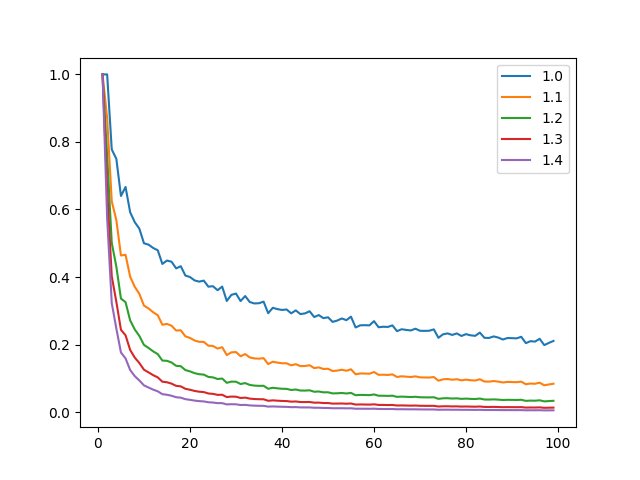
\includegraphics[width=0.95\linewidth]{img/9}			
	\end{multicols}

	A la derecha se encuentran las gráficas para el valor máximo $\ell=8$. El $d$ para el que, en el último $n$, la medida de Hausdorff fue menor que $\varepsilon$, fue $d=1.40\pm0.01$. Ese es el valor que proporciona nuestro algoritmo. Con mayor capacidad de cómputo, haría tender al valor real de $\frac{\log 3}{\log 2} \approx 1.59 \pm 0.01$.
	
	Con este algoritmo, no solo hemos calculado aproximadamente la dimensión de Hausdorff del triángulo de Sierpinski, sino que también podemos calcular la dimensión de otros fractales, incluso de aquellos para los que no tenemos una respuesta teórica.
	
	\newpage
	\section{Código}\label{codigo}
	
	\lstinputlisting[language=Python]{p1vol_rmc.py}
	
\end{document}
